\chapter{MagicDrawToGamma}

A MagicDrawToGamma egy MagicDrawhoz készített állapottérkép verifikációs eszköz, amely formális módszerek segítségével képes ellenőrizni, hogy a rendszer teljesíti-e a felhasználók által megfogalmazott tulajdonságokat.

\section{Plugin működése}

A plugin legfőbb feladata SysML állapottérképek letranszformálása olyan modellekké, melyekhez a formális verifikáció elvégzése már támogatva van, persze mindezt a szemantika megtartása mellett. A Gamma Statechart Composition framework állapottérképek modellezését teszi lehetővé egy saját maga által definiált DSL segítségével. A Gamma képes a modellekből egy olyan .xml alapú dokumentumot generálni amit az UPPAAL nevű eszköz képes feldogozni és az ezek által leírt UPPAAL modelleken formális verifikációt végrehajtani. Az eredményt, azaz az ellenpéldákat, ha vannak, a Gamma képes feldolgozni és visszavezetni a Gamma modellekbe, ezt back-annotationnak nevezik.

A plugin a verifikáció első lépéseként a SysML állapottérképeket Gamma állapottérképekké alakítja, majd a Gamma funkcionalitását kihasználva létrehozza azokat az .xml formátomú dokumentumkat, melyeket az UPPAAL képes feldolgozni. Ezeket az ellenőrizendő tulajdonságokkal együtt az UPPAAL beolvassa és elvégzi a formális verifikációt, aminek eredménye (teljesültek a követelmények vagy sem) megjelenítésre kerülnek.

\begin{figure}[!ht]
	\centering
	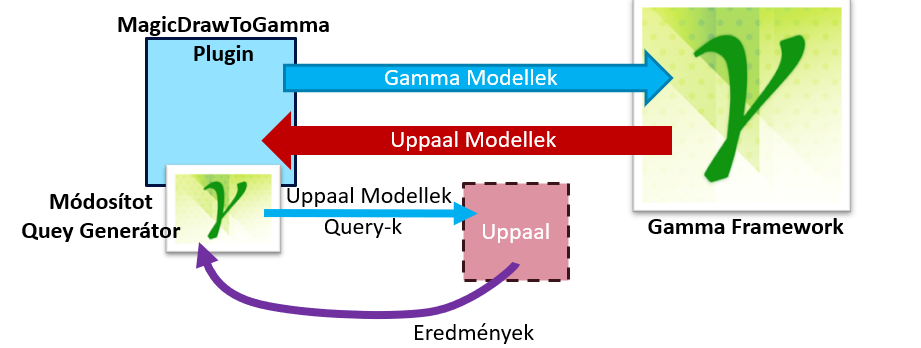
\includegraphics[width=100mm, keepaspectratio]{figures/concept.png}
	\caption{A plugin működése}
	\label{fig:concept}
\end{figure}

A plugin egyenlőre a back-annotationból származó információkat nem képes megjeleníteni, és csak single component állapottérképek transzformációjára képes.







